% Task 6: the leaked table with salt (real salts and digests from leaked_users.txt).
\documentclass[12pt,tikz,border=6pt]{standalone}
% Shared preamble of the task figures of Lecture 7. The colours are the colour roles of the slides
% (main.tex) and of the passwords simulator:
%   Alice sIndigo, Mallory sPink, message / document / password sViolet, salt sAmber,
%   Bob / the server / the notary sTeal, digest sBrown; mechanisms dark; the unknown: orange dashed.
\usepackage{lmodern}
\usepackage[T1]{fontenc}
\renewcommand{\familydefault}{\sfdefault}
\usepackage{amsmath,amssymb}
\usepackage{xcolor}
\usepackage{fontawesome5}
\usetikzlibrary{arrows.meta, calc, positioning, fit, decorations.pathreplacing, backgrounds}

\definecolor{DeepBlue}{HTML}{283593}
\definecolor{AccentOrange}{HTML}{EB5A14}
\definecolor{nInk}{HTML}{37474F}
\definecolor{nLine}{HTML}{90A4AE}
\definecolor{nLight}{HTML}{CFD8DC}
\definecolor{nFill}{HTML}{ECEFF1}
\definecolor{aExec}{HTML}{43A047}
\definecolor{aWrite}{HTML}{E53935}
\definecolor{sIndigo}{HTML}{5C6BC0}
\definecolor{sPink}{HTML}{EC407A}
\definecolor{sViolet}{HTML}{7E57C2}
\definecolor{sAmber}{HTML}{FFB300}
\definecolor{sTeal}{HTML}{26A69A}
\definecolor{sBrown}{HTML}{8D6E63}
\definecolor{sPinkText}{HTML}{C2185B}
\definecolor{sAmberText}{HTML}{A06A00}
\definecolor{sTealText}{HTML}{00796B}

\tikzset{
  hw/.style={draw=nLine, thick, fill=nFill, text=nInk, rounded corners=3pt, align=center, inner sep=4pt},
  mech/.style={draw=nInk, thick, fill=nInk, text=white, rounded corners=3pt, align=center, inner sep=5pt, font=\small\bfseries},
  msgval/.style={draw=sViolet, thick, fill=sViolet!12, text=nInk, rounded corners=3pt, align=center, inner sep=4pt},
  saltval/.style={draw=sAmber, thick, fill=sAmber!25, text=nInk, rounded corners=3pt, align=center, inner sep=4pt},
  digval/.style={draw=sBrown, thick, fill=sBrown!15, text=nInk, rounded corners=3pt, align=center, inner sep=4pt},
  srvval/.style={draw=sTeal, thick, fill=sTeal!15, text=nInk, rounded corners=3pt, align=center, inner sep=4pt},
  unk/.style={draw=AccentOrange, thick, dashed, fill=white, text=AccentOrange, rounded corners=3pt, align=center,
    inner sep=4pt, font=\bfseries},
  data/.style={-{Stealth}, very thick, nInk},
  person/.style={circle, fill=#1, draw=#1, text=white, minimum size=1.1cm, font=\Large, inner sep=0pt},
}
\newcommand{\personnode}[4]{%
  \node[person=#3] (#1) at (#2) {\faUser};
  \node[font=\small\bfseries, text=#3, below=0.06cm of #1] (#1lbl) {#4};}
\newcommand{\mallorynode}[2]{%
  \node[person=sPink] (#1) at (#2) {\faUserSecret};
  \node[font=\small\bfseries, text=sPinkText, below=0.06cm of #1] (#1lbl) {Mallory};}
\newcommand{\hashbox}[4]{\node[mech, minimum width=#4] (#1) at (#2) {\faCogs\ #3};}

\begin{document}
\pagecolor{white}
\begin{tikzpicture}[>=Stealth]
  \node[font=\small\bfseries, text=nInk] at (0,0.6) {user};
  \node[font=\small\bfseries, text=sAmberText] at (2.9,0.6) {salt (public)};
  \node[font=\small\bfseries, text=nInk] at (6.5,0.6) {SHA-256(salt + password)};
  \foreach \u/\s/\d [count=\k from 0] in {alice/a54dca182530bb1d/27b9f609667f414e, carol/3460be31201e69fe/d1d5d3c780e63250, dave/7c2999fdafe59325/04c4b03e1951548b} {
    \node[hw, minimum width=1.6cm, font=\small] at (0,{-0.6*\k}) {\u};
    \node[saltval, minimum width=3.4cm, font=\scriptsize\ttfamily] at (2.9,{-0.6*\k}) {\s\ldots};
    \node[digval, minimum width=3.6cm, font=\scriptsize\ttfamily] at (6.5,{-0.6*\k}) {\d\ldots};
  }
  \node[font=\small, text=gray] at (3.2,-2.0) {\ldots\ the same 12 users as in Task 5};
  \node[mech, font=\scriptsize\bfseries] (h) at (2.9,-3.3) {\faCogs\ SHA-256(salt of user u + guess)};
  \node[msgval, font=\scriptsize\ttfamily] (w) at (-1.4,-3.3) {wordlist.txt};
  \draw[data] (w) -- (h);
  \node[unk, font=\small] at (7.6,-3.3) {cracked: ? of 12\\ SHA-256 computations: ?};
  \draw[data] (h) -- (6.0,-3.3);
  \node[font=\scriptsize, text=nInk, align=left, anchor=west] at (-2.2,-4.3) {For every user: every guess again, with that user's salt. Compare with Task 5: 3\,529 computations.};
\end{tikzpicture}
\end{document}
